\documentclass[border=0.8ex,svgnames,tikz]{standalone}
\usepackage{amsmath,mathtools}
\usepackage{fontspec}
\setmainfont{Source Serif 4}
\setsansfont{Source Sans 3}
\setmonofont{Source Code Pro}
\usetikzlibrary{calc,positioning}
\begin{document}
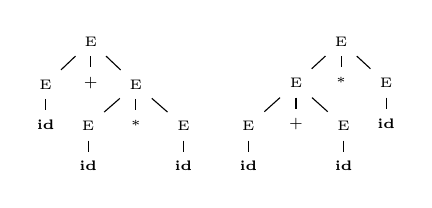
\begin{tikzpicture}
  % a
  \node[](aid1){\tiny \textbf{id}};
  \node[right=21pt of aid1](aid2){\tiny \textbf{id}};
  \node[above=4pt of aid1](aE1){\tiny E};
  \node[above=4pt of aid2](aE2){\tiny E};
  \node[above=-5pt of $(aE1)!0.5!(aE2)$](amul){\tiny *};
  \node[above=4pt of amul](aE3){\tiny E};
  \node[left=21pt of aE3](aE4){\tiny E};
  \node[above=-5pt of $(aE3)!0.5!(aE4)$](aadd){\tiny +};
  \node[below=4pt of aE4](aid3){\tiny \textbf{id}};
  \node[above=4pt of aadd](aE5){\tiny E};
  \path[-]
  (aE5) edge (aE4)
  (aE5) edge (aE3)
  (aE5) edge (aadd)
  (aE4) edge (aid3)
  (aE3) edge (aE2)
  (aE3) edge (aE1)
  (aE3) edge (amul)
  (aE2) edge (aid2)
  (aE1) edge (aid1);

  % b
  \node[right=10pt of aid2](bid1){\tiny \textbf{id}};
  \node[right=21pt of bid1](bid2){\tiny \textbf{id}};
  \node[above=4pt of bid1](bE1){\tiny E};
  \node[above=4pt of bid2](bE2){\tiny E};
  \node[above=-5pt of $(bE1)!0.5!(bE2)$](badd){\tiny +};
  \node[above=4pt of badd](bE3){\tiny E};
  \node[right=21pt of bE3](bE4){\tiny E};
  \node[above=-5pt of $(bE3)!0.5!(bE4)$](bmul){\tiny *};
  \node[below=4pt of bE4](bid3){\tiny \textbf{id}};
  \node[above=4pt of bmul](bE5){\tiny E};
  \path[-]
  (bE5) edge (bE4)
  (bE5) edge (bE3)
  (bE5) edge (bmul)
  (bE4) edge (bid3)
  (bE3) edge (bE2)
  (bE3) edge (bE1)
  (bE3) edge (badd)
  (bE2) edge (bid2)
  (bE1) edge (bid1);
\end{tikzpicture}
\end{document}
